\documentclass[11pt,a4paper]{article}

% ── Packages ──
\usepackage[utf8]{inputenc}
\usepackage[T1]{fontenc}
\usepackage[margin=1in]{geometry}
\usepackage{amsmath,amssymb,amsthm,mathtools}
\usepackage{bm}
\usepackage{xcolor}
\usepackage{hyperref}
\usepackage{listings}
\usepackage{booktabs}
\usepackage{enumitem}
\usepackage{tcolorbox}
\usepackage{tikz}
\usetikzlibrary{arrows.meta,positioning,fit,backgrounds,shapes.geometric,calc}
\usepackage{pgfplots}
\pgfplotsset{compat=1.18}
\usepackage{longtable}
\usepackage{tabularx}
\usepackage{multirow}

\hypersetup{colorlinks=true,linkcolor=blue!70!black,citecolor=green!50!black,urlcolor=blue!60!black}

% ── Code style ──
\lstset{
  language=Python,
  basicstyle=\ttfamily\small,
  keywordstyle=\color{blue!70!black}\bfseries,
  commentstyle=\color{green!50!black}\itshape,
  stringstyle=\color{red!60!black},
  showstringspaces=false,
  breaklines=true,
  frame=single,
  backgroundcolor=\color{gray!5},
  numbers=left,
  numberstyle=\tiny\color{gray},
  xleftmargin=2em,
  framexleftmargin=1.5em
}

% ── Custom boxes ──
\newtcolorbox{action}[1]{colback=green!3,colframe=green!60!black,title={\small\textsc{Action Item:} #1}}
\newtcolorbox{decision}[1]{colback=orange!5,colframe=orange!60!black,title={\small\textsc{Decision Point:} #1}}
\newtcolorbox{mathbox}[1]{colback=blue!3,colframe=blue!50!black,title={\small\textsc{Math to Formalize:} #1}}
\newtcolorbox{code}[1]{colback=purple!3,colframe=purple!50!black,title={\small\textsc{Code to Write:} #1}}
\newtcolorbox{datanote}[1]{colback=teal!3,colframe=teal!50!black,title={\small\textsc{Data:} #1}}
\newtcolorbox{risk}[1]{colback=red!3,colframe=red!50!black,title={\small\textsc{Risk:} #1}}
\newtcolorbox{milestone}{colback=gray!5,colframe=gray!60!black,title={\small\textsc{Milestone / Deliverable}}}

% ── Macros ──
\newcommand{\R}{\mathbb{R}}
\newcommand{\E}{\mathbb{E}}
\newcommand{\Var}{\operatorname{Var}}
\newcommand{\tr}{\operatorname{tr}}
\newcommand{\KL}{\operatorname{KL}}
\newcommand{\ELBO}{\operatorname{ELBO}}
\newcommand{\Normal}{\mathcal{N}}
\newcommand{\HalfCauchy}{\mathrm{C}^{+}}
\newcommand{\Spp}{\mathcal{S}^{+}_p}
\newcommand{\bOmega}{\bm{\Omega}}
\newcommand{\bSigma}{\bm{\Sigma}}

\title{\textbf{Exhaustive Action Plan}\\[0.3em]
\large MCMC vs.\ Variational Inference for Sparse Bayesian Precision Matrix Estimation\\[0.3em]
\normalsize 6.7830 Final Project --- Spring 2026}
\author{Nick Bernardini \and Federico V.\ Cortesi \and Arturo Favara\\
\textit{Massachusetts Institute of Technology}}
\date{Spring 2026}

\begin{document}
\maketitle
\tableofcontents
\clearpage


%======================================================================
%  PART I: PROJECT ARCHITECTURE AND DECISION MAP
%======================================================================
\part{Project Architecture and Decision Map}

\section{Global Overview: What We Are Building}

The project has four interlocking layers, each with multiple route options. Every downstream layer depends on choices made upstream, so we treat the project as a \emph{directed acyclic graph of decisions}.

\begin{figure}[h]
\centering
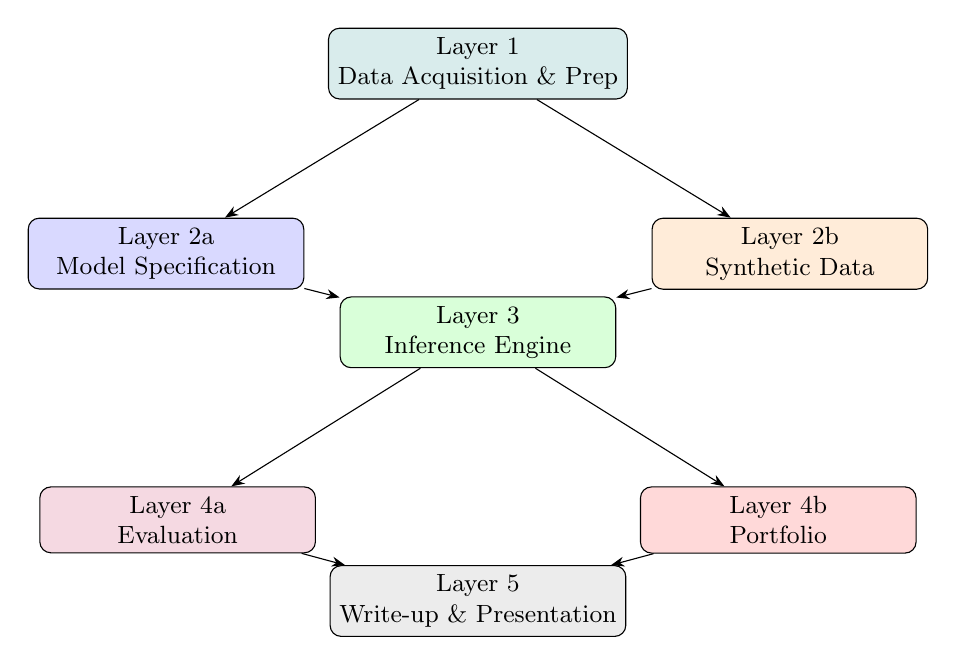
\begin{tikzpicture}[
  block/.style={rectangle, draw, rounded corners, minimum width=3.5cm, minimum height=0.8cm, font=\small, align=center},
  >=Stealth,
  node distance=1.2cm and 0.6cm
]

% Layer 1
\node[block, fill=teal!15] (data) {Layer 1\\Data Acquisition \& Prep};

% Layer 2
\node[block, fill=blue!15, below left=1.5cm and 0.3cm of data] (model) {Layer 2a\\Model Specification};
\node[block, fill=orange!15, below right=1.5cm and 0.3cm of data] (synth) {Layer 2b\\Synthetic Data};

% Layer 3
\node[block, fill=green!15, below=2.5cm of data] (infer) {Layer 3\\Inference Engine};

% Layer 4
\node[block, fill=purple!15, below left=1.5cm and 0.3cm of infer] (eval) {Layer 4a\\Evaluation};
\node[block, fill=red!15, below right=1.5cm and 0.3cm of infer] (port) {Layer 4b\\Portfolio};

% Layer 5
\node[block, fill=gray!15, below=2.5cm of infer] (write) {Layer 5\\Write-up \& Presentation};

\draw[->] (data) -- (model);
\draw[->] (data) -- (synth);
\draw[->] (model) -- (infer);
\draw[->] (synth) -- (infer);
\draw[->] (infer) -- (eval);
\draw[->] (infer) -- (port);
\draw[->] (eval) -- (write);
\draw[->] (port) -- (write);
\end{tikzpicture}
\caption{The five-layer project dependency graph.}
\end{figure}


\section{Master Decision Tree}

At each layer, we face branching choices. The following tree enumerates every major fork. Bolded branches are our \emph{default path}; non-bold are contingency or extension routes.

\subsection{Layer 1: Data}

\begin{decision}{What return data to use?}
\begin{enumerate}[nosep]
  \item[\textbf{(a)}] \textbf{CRSP daily stock returns from WRDS} (our default).
  \item[(b)] Kenneth French's data library (Fama--French factor portfolios, industry returns).
  \item[(c)] Yahoo Finance / free API data (if WRDS access is problematic).
  \item[(d)] ETF returns (sector ETFs as proxy for industry groups).
  \item[(e)] International equity data (for cross-market generalization).
  \item[(f)] Cryptocurrency returns (extreme non-Gaussianity stress test).
\end{enumerate}
\end{decision}

\begin{decision}{What residual preprocessing?}
\begin{enumerate}[nosep]
  \item[\textbf{(a)}] \textbf{Raw demeaned + standardized returns} (default).
  \item[(b)] Fama--French 3-factor residuals (regression on $\text{MKT}, \text{SMB}, \text{HML}$).
  \item[(c)] Fama--French 5-factor + momentum residuals.
  \item[(d)] PCA-based factor residuals (data-driven factors).
  \item[(e)] GARCH-filtered residuals (remove conditional heteroskedasticity first).
\end{enumerate}
\end{decision}

\subsection{Layer 2: Model}

\begin{decision}{Which Bayesian model for $\bOmega$?}
\begin{enumerate}[nosep]
  \item[\textbf{(a)}] \textbf{Graphical horseshoe} (Li, Craig, Bhadra 2019) --- our core model.
  \item[(b)] Bayesian graphical lasso (Wang 2012) --- Laplace prior comparison.
  \item[(c)] Spike-and-slab prior on $\omega_{ij}$ --- gold standard, combinatorially expensive.
  \item[(d)] Finnish horseshoe / regularized horseshoe (Piironen \& Vehtari 2017).
  \item[(e)] Dirichlet--Laplace prior (Bhattacharya et al.\ 2015).
  \item[(f)] R2-D2 prior (Zhang et al.\ 2022).
\end{enumerate}
\end{decision}

\begin{decision}{How to handle the positive-definiteness constraint $\bOmega \succ 0$?}
\begin{enumerate}[nosep]
  \item[\textbf{(a)}] \textbf{Direct parameterization} with MultivariateNormal(precision\_matrix=...).
  \item[(b)] Cholesky reparameterization: $\bOmega = \bm{L}\bm{L}^\top$.
  \item[(c)] Matrix logarithm: work in $\log(\bOmega)$ space (unconstrained symmetric).
  \item[(d)] LKJ base + horseshoe perturbation (hybrid approach).
  \item[(e)] Barrier / potential function penalty for non-PD proposals.
\end{enumerate}
\end{decision}

\subsection{Layer 3: Inference}

\begin{decision}{Which MCMC method?}
\begin{enumerate}[nosep]
  \item[\textbf{(a)}] \textbf{NUTS via NumPyro} (gradient-based, our primary).
  \item[(b)] Li et al.'s custom Gibbs sampler (R or Python port).
  \item[(c)] Metropolis-within-Gibbs (simple but slow mixing).
  \item[(d)] Riemannian HMC (NumPyro does not natively support; would need custom kernel).
  \item[(e)] Sequential Monte Carlo (SMC) samplers via NumPyro.
  \item[(f)] Parallel tempering / replica exchange.
\end{enumerate}
\end{decision}

\begin{decision}{Which VI method?}
\begin{enumerate}[nosep]
  \item[\textbf{(a)}] \textbf{ADVI mean-field} (AutoNormal in NumPyro).
  \item[\textbf{(b)}] \textbf{ADVI full-rank} (AutoMultivariateNormal in NumPyro).
  \item[(c)] AutoLowRankMultivariateNormal (low-rank + diagonal covariance).
  \item[(d)] AutoDelta (MAP estimation, degenerate VI).
  \item[(e)] Structured guide grouping $(\omega_{ij}, \lambda_{ij})$ pairs.
  \item[(f)] Normalizing flow guide (AutoIAFNormal or custom).
  \item[(g)] Stein variational gradient descent (SVGD).
\end{enumerate}
\end{decision}


\subsection{Layer 4: Evaluation \& Application}

\begin{decision}{Which evaluation metrics?}
\begin{enumerate}[nosep]
  \item[\textbf{(a)}] \textbf{Stein's loss, Frobenius loss, spectral norm loss} (primary).
  \item[\textbf{(b)}] \textbf{Sparsity recovery: TPR, FPR, MCC, F1, AUC-ROC} (for synthetic data).
  \item[(c)] Posterior calibration: coverage of 95\% credible intervals.
  \item[(d)] PSIS-diagnostic comparison (Pareto $\hat{k}$) between VI and MCMC.
  \item[(e)] Wasserstein distance between MCMC and VI posteriors.
  \item[(f)] Log predictive density on held-out data.
  \item[(g)] Eigenvalue spectrum overlap (KS test on empirical eigenvalue distributions).
\end{enumerate}
\end{decision}

\begin{decision}{Which portfolio application?}
\begin{enumerate}[nosep]
  \item[\textbf{(a)}] \textbf{Global minimum variance portfolio} (primary).
  \item[(b)] Mean--variance tangency portfolio (requires expected return estimates).
  \item[(c)] Risk parity portfolio ($w_i \propto 1/\sigma_i$, depends on $\bSigma$).
  \item[(d)] Maximum diversification portfolio.
  \item[(e)] Equal-weight (1/N) as a naive baseline.
  \item[(f)] Black--Litterman with Bayesian $\bOmega$ as an input.
\end{enumerate}
\end{decision}


%======================================================================
%  PART II: PHASE-BY-PHASE ACTION PLAN
%======================================================================
\part{Phase-by-Phase Action Plan}

%======================================================================
\section{Phase 0: Environment Setup (Days 1--2)}\label{sec:phase0}
%======================================================================

\begin{action}{Set up the computational environment}
\begin{enumerate}
  \item \textbf{Python environment}: Create a \texttt{conda} or \texttt{venv} environment with Python 3.11+.
  \item \textbf{Core packages}: Install \texttt{jax}, \texttt{jaxlib} (GPU version if available), \texttt{numpyro}, \texttt{arviz}, \texttt{scikit-learn}, \texttt{pandas}, \texttt{numpy}, \texttt{matplotlib}, \texttt{seaborn}.
  \item \textbf{Optional packages}: \texttt{networkx} (graph visualization), \texttt{statsmodels} (factor regressions), \texttt{wrds} (WRDS Python API), \texttt{yfinance} (backup data source).
  \item \textbf{Version control}: Initialize a Git repo; agree on branch strategy (feature branches per team member, merge to \texttt{main}).
  \item \textbf{Hardware}: Confirm GPU access (MIT Engaging cluster, Google Colab Pro, or local GPU). NUTS on $p=100$ may need $>$16 GB GPU RAM.
\end{enumerate}
\end{action}

\begin{code}{Environment setup script}
\begin{lstlisting}
# environment.yml (conda)
name: ggm_horseshoe
channels:
  - conda-forge
dependencies:
  - python=3.11
  - jax
  - jaxlib
  - numpyro
  - arviz
  - scikit-learn
  - pandas
  - numpy
  - matplotlib
  - seaborn
  - networkx
  - statsmodels
  - pip:
    - wrds
    - yfinance
\end{lstlisting}
\end{code}

\begin{action}{Project directory structure}
\begin{lstlisting}[language=bash]
project/
  data/
    raw/          # CRSP downloads, FF factors
    processed/    # cleaned return matrices
    synthetic/    # generated Omega, Y pairs
  src/
    models/       # NumPyro model definitions
    inference/    # NUTS, ADVI, Gibbs runners
    benchmarks/   # Glasso, LW, sample cov
    evaluation/   # loss functions, sparsity metrics
    portfolio/    # GMV, rolling backtest
    utils/        # matrix assembly, plotting helpers
  notebooks/      # exploratory analysis
  results/        # saved posteriors, metric tables
  figures/        # publication-quality plots
  paper/          # LaTeX source for final report
  tests/          # unit tests
\end{lstlisting}
\end{action}

\begin{milestone}
\textbf{End of Phase 0}: Environment runs, imports work, GPU confirmed, repo initialized, directory structure in place.
\end{milestone}


%======================================================================
\section{Phase 1: Data Acquisition and Preprocessing (Days 2--5)}\label{sec:phase1}
%======================================================================

\subsection{Step 1.1: Acquire CRSP Data}

\begin{datanote}{CRSP daily stock file from WRDS}
\begin{enumerate}
  \item \textbf{WRDS query}: Pull CRSP daily returns (\texttt{dsf} table) for NYSE/AMEX/NASDAQ common stocks (\texttt{shrcd} $\in$ \{10, 11\}), date range 2015--2025, fields: \texttt{permno}, \texttt{date}, \texttt{ret}, \texttt{prc}, \texttt{vol}, \texttt{shrout}.
  \item \textbf{Universe selection criteria} (options):
  \begin{enumerate}[nosep]
    \item[(i)] Top $p$ by average daily dollar volume (our default).
    \item[(ii)] S\&P 500 constituents at a fixed date.
    \item[(iii)] Random sample of $p$ stocks with $>$95\% data availability.
    \item[(iv)] Sector-stratified sample (e.g., 10 stocks from each of 10 GICS sectors for $p=100$).
  \end{enumerate}
  \item \textbf{Missing data handling} (options):
  \begin{enumerate}[nosep]
    \item[(i)] Drop any stock with $>$5\% missing days in the estimation window.
    \item[(ii)] Forward-fill up to 3 consecutive missing days, drop the rest.
    \item[(iii)] Use only stocks with complete data in every window (most restrictive, cleanest).
  \end{enumerate}
\end{enumerate}
\end{datanote}

\begin{code}{WRDS data pull}
\begin{lstlisting}
import wrds

db = wrds.Connection()

query = """
SELECT a.permno, a.date, a.ret, a.prc, a.vol, a.shrout
FROM crsp.dsf AS a
INNER JOIN crsp.msenames AS b
  ON a.permno = b.permno
  AND a.date >= b.namedt
  AND a.date <= b.nameendt
WHERE b.shrcd IN (10, 11)
  AND b.exchcd IN (1, 2, 3)
  AND a.date >= '2015-01-01'
  AND a.date <= '2025-12-31'
"""
df = db.raw_sql(query)
df.to_parquet("data/raw/crsp_daily.parquet")
\end{lstlisting}
\end{code}

\subsection{Step 1.2: Alternative / Backup Data Sources}

\begin{datanote}{Options if WRDS is unavailable or for robustness checks}
\begin{enumerate}
  \item \textbf{Yahoo Finance} via \texttt{yfinance}: Free, but survivorship-biased (only currently listed tickers). Good for quick prototyping.
  \item \textbf{Kenneth French Data Library}: Industry portfolio returns (e.g., 49 industry portfolios). Advantage: pre-aggregated, no missing data. Disadvantage: not individual stocks.
  \item \textbf{Quandl / Nasdaq Data Link}: Alternative paid data source.
  \item \textbf{Simulated factor model data}: Generate returns from $\bm{y}_t = \bm{B}\bm{f}_t + \bm{\epsilon}_t$ with known $\bm{B}$, $\bm{\Psi}$, giving known $\bOmega$ for validation.
\end{enumerate}
\end{datanote}

\subsection{Step 1.3: Preprocessing Pipeline}

\begin{action}{Preprocessing steps to implement}
\begin{enumerate}
  \item \textbf{Return computation}: If using price data, compute log returns $r_t = \log(P_t/P_{t-1})$ or simple returns $r_t = P_t/P_{t-1} - 1$. Simple returns are standard for CRSP.
  \item \textbf{Demeaning}: Subtract the sample mean of each stock over the estimation window. \emph{Mathematically}: $\tilde{y}_{k,i} = y_{k,i} - \bar{y}_i$ where $\bar{y}_i = T^{-1}\sum_k y_{k,i}$.
  \item \textbf{Standardization} (decision):
  \begin{enumerate}[nosep]
    \item[(i)] \textbf{Full standardization}: divide by sample std. Advantage: puts all stocks on the same scale; the precision matrix becomes a partial correlation matrix. Disadvantage: loses variance information.
    \item[(ii)] Demean only (no division by std). Advantage: preserves relative volatilities. Disadvantage: large-vol stocks dominate the likelihood.
    \item[(iii)] Robust standardization: divide by MAD (median absolute deviation). More robust to outliers.
  \end{enumerate}
  \item \textbf{Outlier treatment} (options):
  \begin{enumerate}[nosep]
    \item[(i)] Winsorize at 1\%/99\%.
    \item[(ii)] Truncate at $\pm 5\sigma$.
    \item[(iii)] No treatment (let the model handle it; a robustness check).
  \end{enumerate}
  \item \textbf{Rolling windows}: Implement a function that, given a date $t$ and window length $T$, returns the $(T \times p)$ return matrix $\bm{Y}_{[t-T, t)}$.
\end{enumerate}
\end{action}

\begin{mathbox}{Formalize the data model}
Write down explicitly:
\begin{itemize}[nosep]
  \item The assumed data-generating process: $\bm{y}_k \stackrel{\text{iid}}{\sim} \Normal(\bm{0}, \bOmega^{-1})$, $k=1,\ldots,T$.
  \item The sufficient statistic: $\bm{S} = \sum_{k=1}^T \bm{y}_k \bm{y}_k^\top = T \hat{\bSigma}$ (when data is demeaned).
  \item State clearly the assumptions: zero mean, stationarity within the window, Gaussianity, independence across time.
  \item Formally define the concentration ratio: $\gamma = p / T$.
  \item Write out the parameter space: $\bOmega \in \Spp = \{\bm{A} \in \R^{p \times p} : \bm{A} = \bm{A}^\top,\; \bm{A} \succ 0\}$.
\end{itemize}
\end{mathbox}

\subsection{Step 1.4: Factor Model Residuals (Extension Route)}

\begin{action}{Fama--French residual extraction (if pursuing this route)}
\begin{enumerate}
  \item Download daily Fama--French factors from the Kenneth French Data Library.
  \item For each stock $i$, run a time-series regression:
  \begin{equation}
    r_{i,t} - r_{f,t} = \alpha_i + \beta_i^{\text{MKT}}(r_{m,t} - r_{f,t}) + \beta_i^{\text{SMB}}\text{SMB}_t + \beta_i^{\text{HML}}\text{HML}_t + \epsilon_{i,t}.
  \end{equation}
  \item Collect residuals $\hat{\epsilon}_{i,t}$ and form the residual matrix $\hat{\bm{E}} \in \R^{T \times p}$.
  \item Apply the horseshoe to $\hat{\bm{E}}$ instead of raw returns.
  \item \textbf{Justification}: Residuals should have a sparser precision matrix because factor-mediated links have been removed.
  \item \textbf{Caveat}: Estimated residuals introduce additional noise; formally, we should account for the uncertainty in $\hat\beta$ (two-stage estimation problem).
\end{enumerate}
\end{action}

\begin{milestone}
\textbf{End of Phase 1}: Clean $(T \times p)$ return matrices stored for each $(p, T)$ combination. Unit test: verify $\hat\bSigma$ has $\min(\text{rank}, p) = \min(T-1, p)$, and $\hat\bSigma$ is PSD.
\end{milestone}


%======================================================================
\section{Phase 2: Synthetic Data and Ground Truth (Days 3--7)}\label{sec:phase2}
%======================================================================

\subsection{Step 2.1: Generate Known Sparse Precision Matrices}

\begin{mathbox}{Formalize the synthetic data DGP}
We need $\bOmega_0 \in \Spp$ with known sparsity pattern $\mathcal{E}_0 = \{(i,j) : \omega_{ij}^{(0)} \neq 0,\; i \neq j\}$. Define:
\begin{itemize}[nosep]
  \item Sparsity level: $s = |\mathcal{E}_0| / \binom{p}{2} \in [0,1]$.
  \item Edge set generation: choose $\lfloor s \cdot p(p-1)/2 \rfloor$ upper-triangular positions uniformly at random.
  \item Edge weights: sample $\omega_{ij}^{(0)} \sim \text{Uniform}([\text{-}0.8, \text{-}0.3] \cup [0.3, 0.8])$ for $(i,j) \in \mathcal{E}_0$.
  \item Diagonal loading: set $\omega_{ii}^{(0)} = 1$ initially, then adjust to ensure $\bOmega_0 \succ 0$ by adding $(\delta - \lambda_{\min}(\bOmega_0))\bm{I}$ for some margin $\delta > 0$.
  \item Sample data: $\bm{y}_k \sim \Normal(\bm{0}, \bOmega_0^{-1})$ for $k=1,\ldots,T$.
\end{itemize}
\end{mathbox}

\begin{decision}{Which graph structures to test?}
\begin{enumerate}[nosep]
  \item[\textbf{(a)}] \textbf{Erd\H{o}s--R\'enyi random graph}: Each edge included independently with probability $s$. Simple, unstructured.
  \item[(b)] \textbf{Band matrix}: $\omega_{ij} \neq 0$ only if $|i-j| \leq k$ for some bandwidth $k$. Models local dependencies (e.g., similar-sector stocks).
  \item[(c)] \textbf{Block-diagonal}: $K$ blocks of size $p/K$, sparse within blocks, zero between blocks. Models sector structure.
  \item[(d)] \textbf{Star graph}: One hub node connected to all others. Models a ``market factor'' stock.
  \item[(e)] \textbf{Scale-free / power-law graph}: Few high-degree hubs, many low-degree nodes. More realistic for financial networks.
  \item[(f)] \textbf{Small-world graph}: High clustering, short path lengths. (Watts--Strogatz model.)
\end{enumerate}
\end{decision}

\begin{code}{Multiple graph structure generators}
\begin{lstlisting}
import numpy as np
import networkx as nx

def sparse_omega_erdos_renyi(p, s, seed=42):
    G = nx.erdos_renyi_graph(p, s, seed=seed)
    return _graph_to_omega(G, p, seed)

def sparse_omega_band(p, bandwidth=2, seed=42):
    G = nx.Graph()
    G.add_nodes_from(range(p))
    for i in range(p):
        for j in range(i+1, min(i+bandwidth+1, p)):
            G.add_edge(i, j)
    return _graph_to_omega(G, p, seed)

def sparse_omega_block(p, n_blocks=5, intra_sparsity=0.3, seed=42):
    block_size = p // n_blocks
    G = nx.Graph()
    G.add_nodes_from(range(p))
    rng = np.random.default_rng(seed)
    for b in range(n_blocks):
        start = b * block_size
        end = start + block_size
        for i in range(start, end):
            for j in range(i+1, end):
                if rng.random() < intra_sparsity:
                    G.add_edge(i, j)
    return _graph_to_omega(G, p, seed)

def _graph_to_omega(G, p, seed):
    rng = np.random.default_rng(seed)
    Omega = np.eye(p)
    for (i, j) in G.edges():
        val = rng.choice([-1,1]) * rng.uniform(0.3, 0.8)
        Omega[i, j] = val
        Omega[j, i] = val
    # Ensure PD
    eigmin = np.linalg.eigvalsh(Omega).min()
    if eigmin < 0.1:
        Omega += (0.1 - eigmin) * np.eye(p)
    return Omega
\end{lstlisting}
\end{code}

\subsection{Step 2.2: Synthetic Experiment Grid}

\begin{action}{Define the full synthetic experiment matrix}
\begin{center}
\begin{tabular}{@{}ll@{}}
\toprule
\textbf{Factor} & \textbf{Levels} \\
\midrule
Dimension $p$ & 20 (debugging), 50 (main), 100 (scaling) \\
Sample size $T$ & 30, 75, 120, 250, 500 \\
Sparsity $s$ & 0.05 (very sparse), 0.10 (moderate), 0.20 (mild) \\
Graph structure & Erd\H{o}s--R\'enyi, band, block-diagonal \\
Signal strength & weak ($|\omega_{ij}| \in [0.1, 0.3]$), strong ($|\omega_{ij}| \in [0.3, 0.8]$) \\
Random seeds & 5 independent replications per configuration \\
\midrule
Total configs & $3 \times 5 \times 3 \times 3 \times 2 \times 5 = 1350$ \\
\bottomrule
\end{tabular}
\end{center}
\textbf{Triage}: Not all configurations are equally important. Priority order:
\begin{enumerate}[nosep]
  \item $p=50$, $T \in \{75, 250\}$, Erd\H{o}s--R\'enyi, $s=0.10$, strong signal, 3 seeds $\Rightarrow$ \textbf{6 configs} (core results).
  \item Vary $T$ across all 5 levels for the above $\Rightarrow$ \textbf{15 configs} (scaling curves).
  \item Add $p=100$ at $T=250$ $\Rightarrow$ \textbf{+3 configs} (dimensionality scaling).
  \item Add block-diagonal, band $\Rightarrow$ \textbf{+12 configs} (structure sensitivity).
  \item Full grid only if compute allows.
\end{enumerate}
\end{action}

\begin{mathbox}{Ground-truth quantities to precompute}
For each synthetic $\bOmega_0$, precompute and store:
\begin{enumerate}[nosep]
  \item $\bSigma_0 = \bOmega_0^{-1}$ (true covariance).
  \item True edge set $\mathcal{E}_0$ and its complement $\mathcal{E}_0^c$ (for TPR/FPR computation).
  \item Eigenvalues $\lambda_1(\bOmega_0) \geq \ldots \geq \lambda_p(\bOmega_0)$ (for spectral comparison).
  \item Condition number $\kappa(\bOmega_0) = \lambda_1/\lambda_p$.
  \item True graph Laplacian and graph properties (degree distribution, clustering coefficient).
  \item True GMV portfolio weights $\bm{w}_0^* = \bOmega_0\bm{1} / (\bm{1}^\top\bOmega_0\bm{1})$ and oracle portfolio variance $\sigma_0^2 = 1 / (\bm{1}^\top\bOmega_0\bm{1})$.
\end{enumerate}
\end{mathbox}

\begin{milestone}
\textbf{End of Phase 2}: Synthetic data generator produces $(T \times p)$ matrices with known $\bOmega_0$ for any configuration. Unit test: verify that sample $\hat\bSigma$ has eigenvalues consistent with Mar\v{c}enko--Pastur for $\bOmega_0 = \bm{I}$.
\end{milestone}


%======================================================================
\section{Phase 3: Model Implementation (Days 5--12)}\label{sec:phase3}
%======================================================================

\subsection{Step 3.1: Core Graphical Horseshoe Model in NumPyro}

\begin{mathbox}{Write down the full model formally}
The generative model to implement:
\begin{align}
  \tau &\sim \HalfCauchy(0, \sigma_\tau), \label{eq:plan-tau}\\
  \lambda_{ij} &\sim \HalfCauchy(0, 1), \quad \forall\; i < j, \label{eq:plan-lambda}\\
  z_{ij} &\sim \Normal(0, 1), \quad \forall\; i < j, \label{eq:plan-z}\\
  \omega_{ij} &= z_{ij} \cdot \lambda_{ij} \cdot \tau, \quad \forall\; i < j, \label{eq:plan-omega-nc}\\
  \omega_{ii} &\sim \text{Exponential}(\beta_{\text{diag}}) + \delta_{\text{shift}}, \quad \forall\; i, \label{eq:plan-diag}\\
  \bOmega &= \text{assemble}(\{\omega_{ij}\}), \quad \bOmega \in \Spp, \label{eq:plan-assemble}\\
  \bm{y}_k &\sim \Normal(\bm{0}, \bOmega^{-1}), \quad k = 1,\ldots, T. \label{eq:plan-lik}
\end{align}
Note: Eq.~\eqref{eq:plan-omega-nc} is the \textbf{non-centered parameterization}, critical for NUTS.
\end{mathbox}

\begin{decision}{Diagonal prior: what to use?}
\begin{enumerate}[nosep]
  \item[\textbf{(a)}] \textbf{HalfNormal(5)}: Soft constraint, wide. Our default.
  \item[(b)] Exponential($\beta$): Conjugate to certain Gamma likelihoods. $\beta = 0.5$ is weakly informative.
  \item[(c)] Gamma($\alpha, \beta$): More flexible shape. E.g., Gamma(2, 0.5) has mode at 2.
  \item[(d)] Flat improper prior: $\pi(\omega_{ii}) \propto 1$ for $\omega_{ii} > 0$ (as in Li et al.). Requires care with NUTS.
  \item[(e)] Truncated normal: $\Normal^+(0, \sigma^2)$ with large $\sigma$.
\end{enumerate}
\end{decision}

\begin{decision}{Global shrinkage $\tau$: hyperparameter choice?}
\begin{enumerate}[nosep]
  \item[\textbf{(a)}] \textbf{$\HalfCauchy(0, 1)$}: Standard non-informative (Carvalho et al.\ 2010).
  \item[(b)] $\HalfCauchy(0, \sigma_\tau)$ with $\sigma_\tau = s_0 / ((1 - s_0)\sqrt{T})$: Informative, following Piironen \& Vehtari (2017), where $s_0$ is the expected fraction of nonzero entries.
  \item[(c)] Half-$t_3(0, 1)$: Slightly lighter tails than Cauchy; can improve NUTS geometry.
  \item[(d)] Fix $\tau$ at several values and compare (empirical Bayes approach).
\end{enumerate}
\end{decision}

\begin{code}{Complete model with multiple parameterization options}
\begin{lstlisting}
import jax.numpy as jnp
import numpyro
import numpyro.distributions as dist

def graphical_horseshoe_v1(Y, p,
                            ncp=True,
                            tau_scale=1.0,
                            diag_prior="halfnormal"):
    """
    Version 1: Direct parameterization with PD check.
    ncp: if True, use non-centered parameterization.
    """
    T = Y.shape[0]
    n_offdiag = p * (p - 1) // 2

    # Global shrinkage
    tau = numpyro.sample("tau",
        dist.HalfCauchy(tau_scale))

    # Local shrinkage
    lambdas = numpyro.sample("lambdas",
        dist.HalfCauchy(jnp.ones(n_offdiag)))

    # Off-diagonal elements
    if ncp:
        z = numpyro.sample("z",
            dist.Normal(jnp.zeros(n_offdiag), 1.0))
        omega_offdiag = numpyro.deterministic(
            "omega_offdiag", z * lambdas * tau)
    else:
        omega_offdiag = numpyro.sample(
            "omega_offdiag",
            dist.Normal(0, lambdas * tau))

    # Diagonal
    if diag_prior == "halfnormal":
        omega_diag = numpyro.sample("omega_diag",
            dist.HalfNormal(jnp.ones(p) * 5.0))
    elif diag_prior == "exponential":
        omega_diag = numpyro.sample("omega_diag",
            dist.Exponential(jnp.ones(p) * 0.5))
    elif diag_prior == "gamma":
        omega_diag = numpyro.sample("omega_diag",
            dist.Gamma(2.0 * jnp.ones(p),
                       0.5 * jnp.ones(p)))

    # Assemble
    Omega = jnp.zeros((p, p))
    idx = jnp.triu_indices(p, k=1)
    Omega = Omega.at[idx].set(omega_offdiag)
    Omega = Omega + Omega.T + jnp.diag(omega_diag)

    # Likelihood
    numpyro.sample("Y",
        dist.MultivariateNormal(
            loc=jnp.zeros(p),
            precision_matrix=Omega),
        obs=Y)
\end{lstlisting}
\end{code}

\subsection{Step 3.2: Cholesky Reparameterization (Alternative Route)}

\begin{mathbox}{Cholesky factorization approach}
Instead of assembling $\bOmega$ directly, parameterize via its Cholesky factor:
\begin{equation}
  \bOmega = \bm{L}\bm{L}^\top, \quad L_{ii} > 0, \quad L_{ij} \text{ free for } i > j.
\end{equation}
The horseshoe prior is placed on the off-diagonal entries of $\bm{L}$:
\begin{equation}
  L_{ij} \mid \tilde\lambda_{ij}, \tau \sim \Normal(0, \tilde\lambda_{ij}^2 \tau^2), \quad \tilde\lambda_{ij} \sim \HalfCauchy(0,1).
\end{equation}
\textbf{Advantage}: $\bOmega \succ 0$ is guaranteed by construction.\\
\textbf{Disadvantage}: Sparsity in $\bm{L}$ does not directly correspond to sparsity in $\bOmega = \bm{L}\bm{L}^\top$. The horseshoe shrinks $L_{ij}$ toward zero, but $\omega_{ij} = \sum_k L_{ik}L_{jk}$ is a sum, so individual zeros in $\bm{L}$ do not guarantee zeros in $\bOmega$.
\end{mathbox}

\subsection{Step 3.3: Validation on Trivial Cases}

\begin{action}{Sanity checks before running real experiments}
\begin{enumerate}
  \item \textbf{Wishart posterior recovery}: Set $p=5$, $T=1000$, $\bOmega_0 = \bm{I}$, use a Wishart prior (no horseshoe). Check that NUTS recovers $\bOmega_0$ and that the posterior matches the known Wishart($\nu_0 + T$, $(\bm{V}_0^{-1} + \bm{S})^{-1}$).
  \item \textbf{Small-$p$ horseshoe}: $p=3$, $T=500$, $\bOmega_0 = \text{tridiagonal}$. Run NUTS with 10,000 samples. Check:
  \begin{itemize}[nosep]
    \item Posterior mean close to truth?
    \item Zero entries have posterior mass concentrated near 0?
    \item Non-zero entries have posterior centered near true value?
    \item $\hat{R} < 1.01$ for all parameters?
    \item No divergent transitions?
  \end{itemize}
  \item \textbf{Prior predictive check}: Sample from the prior (no data) and verify that the prior implies reasonable precision matrices (condition numbers not astronomical, eigenvalues not degenerate).
  \item \textbf{Fake data calibration (SBC)}: Simulation-based calibration (Talts et al.\ 2018). For $M=100$ synthetic datasets, check that posterior rank statistics are uniform.
\end{enumerate}
\end{action}

\begin{mathbox}{Simulation-Based Calibration (SBC) protocol}
For each replicate $m=1,\ldots,M$:
\begin{enumerate}[nosep]
  \item Sample $\bOmega^{(m)} \sim \pi(\bOmega)$ from the prior.
  \item Generate $\bm{Y}^{(m)} \sim p(\bm{Y} \mid \bOmega^{(m)})$.
  \item Run NUTS to obtain posterior samples $\{\bOmega^{(m,s)}\}_{s=1}^S$.
  \item Compute rank: $r^{(m)} = \#\{s : \omega_{12}^{(m,s)} < \omega_{12}^{(m)}\}$.
\end{enumerate}
If the inference is well-calibrated, $r^{(m)} \sim \text{Uniform}(\{0,\ldots,S\})$ across replicates.
\end{mathbox}

\begin{milestone}
\textbf{End of Phase 3}: NumPyro model passes all sanity checks. NUTS runs on $p=3$ and $p=20$ synthetic data with good diagnostics ($\hat{R} < 1.01$, bulk ESS $> 400$, no divergences).
\end{milestone}


%======================================================================
\section{Phase 4: Inference at Scale (Days 10--18)}\label{sec:phase4}
%======================================================================

\subsection{Step 4.1: NUTS across the $(p, T)$ Grid}

\begin{action}{NUTS run protocol}
For each $(p, T, \bOmega_0)$ configuration:
\begin{enumerate}
  \item Set \texttt{target\_accept\_prob} = 0.85 (default; increase to 0.95 if divergences appear).
  \item Set \texttt{max\_tree\_depth} = 10 (default; increase to 12 if ESS is low).
  \item Run 4 chains with \texttt{num\_warmup} = 2000, \texttt{num\_samples} = 5000.
  \item Record wall-clock time, \# divergences, min/max $\hat{R}$, min bulk ESS, min tail ESS.
  \item If divergences $>$ 0: try increasing \texttt{target\_accept\_prob}, switching to centered parameterization, or thinning the half-Cauchy to half-$t_3$.
  \item Save posterior samples to disk (HDF5 or \texttt{.npz}).
\end{enumerate}
\end{action}

\begin{decision}{If NUTS fails at $p=100$?}
\begin{enumerate}[nosep]
  \item[\textbf{(a)}] \textbf{Reduce to $p=50$} and report $p=100$ as infeasible for NUTS.
  \item[(b)] Implement Li et al.'s Gibbs sampler as the MCMC baseline for $p=100$.
  \item[(c)] Use fewer warmup/samples (e.g., 500/1000) with a note on convergence quality.
  \item[(d)] Try SMC (Sequential Monte Carlo) in NumPyro as an alternative.
  \item[(e)] Subsample: run NUTS on the sufficient statistic $\bm{S}$ directly (does not reduce per-iteration cost but avoids loading all $T$ rows into memory).
\end{enumerate}
\end{decision}

\subsection{Step 4.2: ADVI (Mean-Field and Full-Rank)}

\begin{action}{ADVI run protocol}
\begin{enumerate}
  \item \textbf{Mean-field ADVI}:
  \begin{itemize}[nosep]
    \item Guide: \texttt{AutoNormal(model)}.
    \item Optimizer: \texttt{Adam(lr=0.01)} with cosine annealing or step decay.
    \item Steps: 50,000 (monitor ELBO convergence; stop early if plateau).
    \item Run from 5 different random seeds to assess initialization sensitivity.
  \end{itemize}
  \item \textbf{Full-rank ADVI}:
  \begin{itemize}[nosep]
    \item Guide: \texttt{AutoMultivariateNormal(model)}.
    \item Optimizer: \texttt{Adam(lr=0.005)} (slower learning rate for stability).
    \item Steps: 100,000.
    \item \textbf{Feasibility check}: For $p=50$, $D \approx 3700$; the full Cholesky of the guide has $D(D+1)/2 \approx 7$M parameters. This may be infeasible. If so, use \texttt{AutoLowRankMultivariateNormal(rank=50)} as a compromise.
  \end{itemize}
  \item \textbf{Diagnostics to record}:
  \begin{itemize}[nosep]
    \item Final ELBO and its standard deviation across seeds.
    \item ELBO trace (convergence curve).
    \item Gradient norm trace (detect explosions).
    \item PSIS diagnostic: use \texttt{arviz} to compute Pareto $\hat{k}$ values by importance-sampling the VI posterior against MCMC.
  \end{itemize}
  \item \textbf{Post-VI sampling}: Draw 5000 samples from the fitted guide for downstream analysis.
\end{enumerate}
\end{action}

\begin{decision}{Learning rate schedule options}
\begin{enumerate}[nosep]
  \item[(a)] Constant \texttt{lr=0.01}.
  \item[(b)] Cosine annealing: \texttt{lr} decays from 0.01 to 0.0001 over the run.
  \item[(c)] Step decay: halve \texttt{lr} every 10,000 steps.
  \item[(d)] Adaptive: use \texttt{ClippedAdam} with gradient clipping at norm 10.
  \item[(e)] Two-phase: 0.01 for first 30k steps, 0.001 for remaining.
\end{enumerate}
\end{decision}

\subsection{Step 4.3: Additional VI Variants (Extension Routes)}

\begin{action}{Optional VI extensions to try}
\begin{enumerate}
  \item \textbf{Structured mean-field}: Write a custom guide that groups $(\omega_{ij}, \lambda_{ij})$ into bivariate Gaussian blocks:
  \begin{equation}
    q(\bm{\theta}) = q(\tau) \prod_{i<j} q_{ij}(\omega_{ij}, \lambda_{ij}),
  \end{equation}
  where each $q_{ij}$ is a bivariate Normal in the unconstrained space.
  \item \textbf{Low-rank ADVI}: \texttt{AutoLowRankMultivariateNormal(model, rank=r)} with $r \in \{10, 25, 50\}$. Captures some correlation structure at $O(Dr)$ cost instead of $O(D^2)$.
  \item \textbf{MAP estimation}: \texttt{AutoDelta(model)} gives the mode of the posterior. Useful as a point estimate baseline but provides no uncertainty quantification.
  \item \textbf{Normalizing flow guide}: If NumPyro supports \texttt{AutoIAFNormal} (inverse autoregressive flow), this can capture multimodality. Expensive but potentially recovers the bimodal shrinkage.
\end{enumerate}
\end{action}

\subsection{Step 4.4: Frequentist Benchmarks}

\begin{action}{Run all frequentist methods}
\begin{enumerate}
  \item \textbf{Sample covariance}: $\hat\bSigma = (T-1)^{-1}\bm{Y}^\top\bm{Y}$, $\hat\bOmega = \hat\bSigma^{-1}$ (if invertible).
  \item \textbf{Ledoit--Wolf}: \texttt{sklearn.covariance.LedoitWolf}. Record shrinkage intensity $\hat\alpha$.
  \item \textbf{Graphical lasso with CV}: \texttt{sklearn.covariance.GraphicalLassoCV(cv=5)}. Record selected $\rho$.
  \item \textbf{Graphical lasso on a grid}: Also run for $\rho \in \{0.01, 0.05, 0.1, 0.2, 0.5, 1.0\}$ to plot the regularization path.
  \item \textbf{Oracle (synthetic only)}: The true $\bOmega_0$ itself (establishes the best possible performance).
  \item \textbf{Nonlinear shrinkage} (optional extension): Ledoit--Wolf (2020) analytical nonlinear shrinkage. Use the \texttt{sklearn\_extra} or custom implementation.
  \item \textbf{POET estimator} (optional): Factor-model-based estimator (Fan, Liao, Mincheva 2013). Use \texttt{factor\_analyzer} or custom PCA + thresholding.
\end{enumerate}
\end{action}

\begin{milestone}
\textbf{End of Phase 4}: All inference methods have run on at least the core configurations. Posterior samples (NUTS, ADVI-MF, ADVI-FR) and point estimates (glasso, LW, sample cov) are saved. Wall-clock times are recorded.
\end{milestone}


%======================================================================
\section{Phase 5: Evaluation and Analysis (Days 15--22)}\label{sec:phase5}
%======================================================================

\subsection{Step 5.1: Point Estimation Losses}

\begin{mathbox}{Loss functions to compute}
For each method $m$ and configuration $(p, T, \bOmega_0)$:
\begin{enumerate}
  \item \textbf{Stein's loss}:
  \begin{equation}
    L_S^{(m)} = \tr\!\big((\hat\bOmega^{(m)})^{-1}\bOmega_0\big) - \log\!\big|(\hat\bOmega^{(m)})^{-1}\bOmega_0\big| - p.
  \end{equation}
  \item \textbf{Frobenius loss}: $L_F^{(m)} = \|\hat\bOmega^{(m)} - \bOmega_0\|_F^2$.
  \item \textbf{Spectral loss}: $L_2^{(m)} = \|\hat\bOmega^{(m)} - \bOmega_0\|_2$.
  \item \textbf{Relative Frobenius}: $L_{F,\text{rel}}^{(m)} = \|\hat\bOmega^{(m)} - \bOmega_0\|_F / \|\bOmega_0\|_F$.
  \item \textbf{Elementwise MAE}: $\text{MAE}^{(m)} = \frac{1}{p^2}\sum_{i,j}|\hat\omega^{(m)}_{ij} - \omega^{(0)}_{ij}|$.
\end{enumerate}
For Bayesian methods, $\hat\bOmega^{(m)}$ is the posterior mean.

Also compute \textbf{posterior median} and \textbf{posterior mode} estimates for robustness.
\end{mathbox}

\subsection{Step 5.2: Sparsity Recovery Analysis}

\begin{action}{Edge detection and ROC analysis}
\begin{enumerate}
  \item \textbf{For the graphical lasso}: Vary $\rho$ over a grid and record (TPR, FPR) pairs $\Rightarrow$ ROC curve.
  \item \textbf{For NUTS/ADVI}: Vary the credible interval level $\alpha \in [0.01, 0.99]$:
  \begin{itemize}[nosep]
    \item Edge $(i,j)$ declared present if $P(|\omega_{ij}| > 0 \mid \bm{Y}) > \alpha$.
    \item Equivalently: the $(1-\alpha)$ credible interval for $\omega_{ij}$ excludes zero.
  \end{itemize}
  This traces out a Bayesian ROC curve.
  \item \textbf{Metrics at a fixed threshold}:
  \begin{itemize}[nosep]
    \item 95\% credible interval criterion (standard choice).
    \item TPR, FPR, MCC, F1, precision, recall.
    \item Number of selected edges vs.\ true edge count.
  \end{itemize}
  \item \textbf{Key comparison}: Does ADVI recover the same graph as NUTS? Compute the edge-set Jaccard similarity between ADVI and NUTS selections.
\end{enumerate}
\end{action}

\subsection{Step 5.3: Shrinkage Profile Analysis}

\begin{mathbox}{Quantifying the shrinkage distortion of VI}
The core diagnostic for our paper's thesis. For each off-diagonal entry $(i,j)$:
\begin{enumerate}
  \item Compute the NUTS posterior shrinkage coefficient:
  \begin{equation}
    \hat\kappa_{ij}^{\text{NUTS}} = \frac{1}{S}\sum_{s=1}^S \frac{1}{1 + (\lambda_{ij}^{(s)})^2 (\tau^{(s)})^2}.
  \end{equation}
  \item Compute the same from ADVI samples.
  \item \textbf{Bimodality test}: Compute the bimodality coefficient $b = (g^2 + 1) / (\kappa + 3(n-1)^2/((n-2)(n-3)))$ where $g$ is skewness and $\kappa$ is excess kurtosis. $b > 5/9$ suggests bimodality.
  \item Plot histograms of $\hat\kappa_{ij}$ across all $(i,j)$ pairs for NUTS vs.\ ADVI side by side. If ADVI's distribution is unimodal while NUTS's is bimodal, we have our main finding.
  \item \textbf{Wasserstein-1 distance} between the empirical distributions of $\{\hat\kappa_{ij}\}$ from NUTS vs.\ ADVI, as a scalar summary of shrinkage distortion.
\end{enumerate}
\end{mathbox}

\subsection{Step 5.4: Posterior Uncertainty Comparison}

\begin{action}{Compare posterior variances}
\begin{enumerate}
  \item For each $\omega_{ij}$, compute $\text{Var}_{\text{NUTS}}[\omega_{ij}]$ and $\text{Var}_{\text{ADVI}}[\omega_{ij}]$.
  \item Plot $\log(\text{Var}_{\text{ADVI}}) / \log(\text{Var}_{\text{NUTS}})$ as a function of $|\hat\omega_{ij}^{\text{NUTS}}|$. We expect ADVI to underestimate variance, especially for entries near zero (where the horseshoe posterior is highly non-Gaussian).
  \item \textbf{Calibration check}: For the synthetic case, compute the coverage of 95\% posterior intervals. Does NUTS achieve 95\%? Does ADVI achieve less?
  \item \textbf{Interval width ratio}: $\text{width}_{\text{ADVI}} / \text{width}_{\text{NUTS}}$ for each $\omega_{ij}$.
\end{enumerate}
\end{action}

\subsection{Step 5.5: Convergence Diagnostics Deep Dive}

\begin{action}{MCMC diagnostics to present}
\begin{enumerate}
  \item \textbf{$\hat{R}$ summary}: Distribution of $\hat{R}$ across all parameters. Report max $\hat{R}$.
  \item \textbf{ESS summary}: Distribution of bulk ESS and tail ESS. Report min ESS.
  \item \textbf{Trace plots}: For $\tau$, a few representative $\lambda_{ij}$, a few $\omega_{ij}$ (one true zero, one true nonzero).
  \item \textbf{Divergence analysis}: If divergences occur, plot the divergent points in parameter space. Do they cluster in the ``funnel'' (low $\lambda_{ij}$ region)?
  \item \textbf{Energy plot}: NumPyro energy diagnostic (marginal vs.\ transitional energy).
  \item \textbf{Pair plots}: Joint posteriors of $(\omega_{ij}, \lambda_{ij})$ for a few entries.
\end{enumerate}
\end{action}

\begin{action}{VI diagnostics to present}
\begin{enumerate}
  \item \textbf{ELBO trace}: Plot ELBO vs.\ iteration for mean-field and full-rank.
  \item \textbf{Multi-seed ELBO}: Overlay 5 runs from different seeds. Spread $\Rightarrow$ initialization sensitivity.
  \item \textbf{ELBO gap}: If we trust NUTS marginal likelihood (via harmonic mean estimator or bridge sampling), compute $\log p(\bm{Y}) - \ELBO_{\text{final}} \approx \KL(q\|p)$.
  \item \textbf{PSIS diagnostics}: Using \texttt{arviz.loo} machinery, compute Pareto $\hat{k}$ values for importance-weighting VI samples toward the MCMC posterior. $\hat{k} > 0.7$ indicates serious approximation failure.
\end{enumerate}
\end{action}

\subsection{Step 5.6: Eigenvalue Spectrum Analysis}

\begin{mathbox}{Spectral comparison}
For each estimator $\hat\bOmega$, compute eigenvalues $\hat\lambda_1 \geq \ldots \geq \hat\lambda_p$ and compare against $\lambda_1^{(0)} \geq \ldots \geq \lambda_p^{(0)}$:
\begin{enumerate}[nosep]
  \item Eigenvalue-by-eigenvalue comparison plot (sorted eigenvalues).
  \item KS test statistic between the empirical eigenvalue distributions.
  \item Condition number comparison: $\hat\kappa = \hat\lambda_1 / \hat\lambda_p$ vs.\ $\kappa_0$.
  \item Trace comparison: $\tr(\hat\bOmega)$ vs.\ $\tr(\bOmega_0)$ (should be close since trace equals sum of diagonal elements).
\end{enumerate}
\end{mathbox}

\begin{milestone}
\textbf{End of Phase 5}: All evaluation tables and plots are generated for synthetic data. Key finding (bimodal shrinkage distortion under VI) is confirmed or refuted.
\end{milestone}


%======================================================================
\section{Phase 6: Portfolio Construction and Financial Application (Days 18--23)}\label{sec:phase6}
%======================================================================

\subsection{Step 6.1: In-Sample GMV Portfolio}

\begin{mathbox}{GMV portfolio from precision matrix}
For each estimator $\hat\bOmega$:
\begin{equation}
  \bm{w}^* = \frac{\hat\bOmega\,\bm{1}}{\bm{1}^\top\hat\bOmega\,\bm{1}}.
\end{equation}
This requires $\hat\bOmega$ to be PD (guaranteed for Bayesian posterior means; may need regularization for sample covariance when $p > T$).

\textbf{Bayesian posterior portfolio distribution}: For NUTS samples $\hat\bOmega^{(1)},\ldots,\hat\bOmega^{(S)}$:
\begin{equation}
  \bm{w}^{(s)} = \frac{\hat\bOmega^{(s)}\bm{1}}{\bm{1}^\top\hat\bOmega^{(s)}\bm{1}}, \quad s=1,\ldots,S.
\end{equation}
This gives a posterior distribution over weights, from which we can compute:
\begin{itemize}[nosep]
  \item Posterior mean weights $\bar{\bm{w}} = S^{-1}\sum_s \bm{w}^{(s)}$ (differs from weights computed from the posterior mean $\bar\bOmega$!).
  \item Weight uncertainty: $\text{sd}(w_i) = \sqrt{S^{-1}\sum_s (w_i^{(s)} - \bar{w}_i)^2}$.
  \item Posterior predictive portfolio variance.
\end{itemize}
\end{mathbox}

\subsection{Step 6.2: Rolling Window Out-of-Sample Backtest}

\begin{action}{Backtesting protocol}
\begin{enumerate}
  \item Fix $p$ and estimation window $T$.
  \item For each rebalancing date $t$ (e.g., monthly):
  \begin{enumerate}[nosep]
    \item[(i)] Extract the in-sample return matrix $\bm{Y}_{[t-T, t)}$.
    \item[(ii)] Estimate $\hat\bOmega$ using each method.
    \item[(iii)] Compute GMV weights $\bm{w}_t^*$.
    \item[(iv)] Record out-of-sample return: $r_t^{\text{pf}} = (\bm{w}_t^*)^\top \bm{r}_t$.
  \end{enumerate}
  \item Over the full backtest period, compute:
  \begin{itemize}[nosep]
    \item Annualized out-of-sample portfolio volatility: $\hat\sigma_{\text{oos}} = \sqrt{252} \cdot \text{std}(\{r_t^{\text{pf}}\})$.
    \item Annualized Sharpe ratio (if using excess returns): $\text{SR} = \sqrt{252} \cdot \bar{r}^{\text{pf}} / \text{std}(r^{\text{pf}})$.
    \item Maximum drawdown.
    \item Turnover: $\text{TO}_t = \sum_i |w_{i,t} - w_{i,t-1}|$.
    \item Average portfolio concentration: Herfindahl index $\text{HHI}_t = \sum_i w_{i,t}^2$.
  \end{itemize}
  \item \textbf{Key comparison}: Which estimator yields the lowest out-of-sample variance?
\end{enumerate}
\end{action}

\begin{decision}{Backtesting frequency and length?}
\begin{enumerate}[nosep]
  \item[\textbf{(a)}] \textbf{Monthly rebalancing} with 1-year estimation window ($T=250$). 5--8 year backtest.
  \item[(b)] Quarterly rebalancing (less data, less rebalancing noise).
  \item[(c)] Weekly rebalancing (more data points, higher turnover).
  \item[(d)] Multiple estimation windows: $T \in \{120, 250, 500\}$ simultaneously.
\end{enumerate}
\end{decision}

\begin{risk}{Backtest computational cost}
Running NUTS for each rebalancing date is expensive. For 60 monthly rebalancing points, each requiring $\sim$30 minutes of NUTS at $p=50$, we need $\sim$30 hours. Strategies:
\begin{enumerate}[nosep]
  \item Run NUTS on a subset of dates (e.g., every 6 months) and interpolate.
  \item Use warm-starting: initialize NUTS at rebalancing date $t$ from the posterior of date $t-1$.
  \item For ADVI, each fit takes $\sim$5 minutes, making the full backtest feasible.
  \item Use only a single representative date for NUTS and full backtest for ADVI + frequentist.
\end{enumerate}
\end{risk}

\subsection{Step 6.3: Bayesian Decision Theory Angle (Extension)}

\begin{mathbox}{Posterior expected loss for portfolio selection}
Instead of using the posterior mean $\bar\bOmega$, we can compute the \emph{Bayes-optimal} portfolio weights under a specific loss function:
\begin{equation}
  \bm{w}^{\text{Bayes}} = \arg\min_{\bm{w}} \E_{p(\bOmega \mid \bm{Y})}\!\big[\bm{w}^\top \bOmega^{-1} \bm{w}\big] \quad \text{s.t.} \quad \bm{w}^\top\bm{1} = 1.
\end{equation}
This is equivalent to $\bm{w}^{\text{Bayes}} = \frac{\bar\bOmega_{\text{inv}}\bm{1}}{\bm{1}^\top\bar\bOmega_{\text{inv}}\bm{1}}$ where $\bar\bOmega_{\text{inv}} = \E[\bOmega^{-1} \mid \bm{Y}] = S^{-1}\sum_s (\bOmega^{(s)})^{-1}$.

\textbf{Note}: $\E[\bOmega^{-1}] \neq (\E[\bOmega])^{-1}$ by Jensen's inequality. This distinction matters.
\end{mathbox}

\begin{milestone}
\textbf{End of Phase 6}: Portfolio backtest results are in. Out-of-sample volatilities are compared across methods. Key question answered: does the Bayesian approach (with uncertainty quantification) produce meaningfully different portfolio behavior?
\end{milestone}


%======================================================================
\section{Phase 7: Real Data Analysis (Days 16--22, overlapping)}\label{sec:phase7}
%======================================================================

\subsection{Step 7.1: Apply All Methods to CRSP Data}

\begin{action}{Real data experiments}
\begin{enumerate}
  \item Select $p=50$ and $p=100$ stock universes.
  \item Choose a representative date (e.g., end of 2023) with $T=250$ (1 year of daily data).
  \item Run all 6 methods: sample cov, LW, glasso, NUTS, ADVI-MF, ADVI-FR.
  \item \textbf{No ground truth}: We cannot compute Stein's loss or Frobenius loss against $\bOmega_0$. Instead:
  \begin{enumerate}[nosep]
    \item[(i)] Compare methods against each other (pairwise Frobenius distances).
    \item[(ii)] Out-of-sample log-likelihood on a held-out test set.
    \item[(iii)] Portfolio performance (the ultimate practical test).
    \item[(iv)] Sparsity patterns: visualize the estimated graph as a network; do the connections make economic sense (e.g., within-sector edges)?
  \end{enumerate}
\end{enumerate}
\end{action}

\subsection{Step 7.2: Sparsity Validation via External Structure}

\begin{action}{Economic plausibility checks}
\begin{enumerate}
  \item \textbf{GICS sector overlay}: Color nodes by sector. Are edges predominantly within-sector? An informative sanity check.
  \item \textbf{Factor exposure correlation}: Do strongly connected stocks share similar Fama--French loadings?
  \item \textbf{Known pairs}: Check whether well-known pairs (e.g., Coca-Cola/PepsiCo, Visa/Mastercard) appear as edges. Are they absent from the conditional graph (as expected if their co-movement is factor-mediated)?
  \item \textbf{Stability analysis}: Run the estimator on two non-overlapping windows and compare the graph structures. How stable are the detected edges?
\end{enumerate}
\end{action}

\subsection{Step 7.3: Fama--French Residual Analysis (Extension Route)}

\begin{action}{Factor-adjusted analysis}
\begin{enumerate}
  \item Regress each stock on FF3 (or FF5+Mom) factors.
  \item Collect residuals and re-run the full pipeline on residual returns.
  \item Compare sparsity patterns: residual graph should be sparser than raw return graph.
  \item Compare estimation losses on held-out data.
\end{enumerate}
\end{action}

\begin{milestone}
\textbf{End of Phase 7}: Real data analysis complete. Estimated graphs are visualized. Portfolio backtests on CRSP data are done. Economic plausibility of the horseshoe estimates is assessed.
\end{milestone}


%======================================================================
\section{Phase 8: Write-up (Days 20--28)}\label{sec:phase8}
%======================================================================

\subsection{Step 8.1: Progress Report (Due April 15)}

\begin{action}{Progress report content (2 pages/member = 6 pages max)}
\begin{enumerate}
  \item \textbf{What's done}: Model implemented, validated on synthetic data, NUTS and ADVI running, preliminary results for core $(p,T)$ configurations.
  \item \textbf{Preliminary findings}: Show one precision matrix heatmap comparison, one shrinkage profile plot, one loss curve. State whether ADVI-MF shows the expected shrinkage distortion.
  \item \textbf{What remains}: Portfolio backtest, real data analysis, remaining configurations, full write-up.
  \item \textbf{Plot description}: Describe the ``loss vs.\ $p/T$'' plot. Horizontal axis: $p/T$ ratio. Vertical axis: Stein's loss. Lines for each method. What will the reader learn: at what $p/T$ do Bayesian methods dominate? Does ADVI degrade faster than NUTS?
\end{enumerate}
\end{action}

\subsection{Step 8.2: Final Report (Due May 5)}

\begin{action}{Final report structure (4 pages/member = 12 pages max)}
We recommend the following sections:
\begin{enumerate}
  \item \textbf{Introduction} (1 page): Problem statement, why precision matrices matter for GGMs and finance, our research question.
  \item \textbf{Model} (1.5 pages): Graphical horseshoe specification with full math. Prior choices and their rationale.
  \item \textbf{Methods} (2 pages): NUTS setup, ADVI setup, frequentist benchmarks. Implementation details that matter for replication.
  \item \textbf{Experiments} (3 pages): Synthetic results (losses, sparsity recovery, shrinkage profiles). Real data results (portfolio backtest, graph structure).
  \item \textbf{Discussion} (1.5 pages): Why does ADVI fail/succeed for the horseshoe? Implications for practitioners. Connection to class themes.
  \item \textbf{Conclusion} (0.5 pages): Summary of findings, limitations, future work.
  \item \textbf{References}: Does not count toward page limit.
\end{enumerate}
\end{action}

\subsection{Step 8.3: Figures to Produce}

\begin{action}{Complete figure list}
\begin{enumerate}
  \item \textbf{Fig 1}: Precision matrix heatmaps (6 panels: truth, sample cov, LW, glasso, NUTS, ADVI-MF). One $(p,T)$ configuration.
  \item \textbf{Fig 2}: Shrinkage profile histograms (NUTS vs.\ ADVI-MF vs.\ ADVI-FR). $x$-axis: $|\hat\omega_{ij}|$ (or $\hat\kappa_{ij}$). Main finding figure.
  \item \textbf{Fig 3}: Loss vs.\ $p/T$ curves (Stein's loss, Frobenius). With error bars from multiple seeds.
  \item \textbf{Fig 4}: ROC curves for graph recovery.
  \item \textbf{Fig 5}: ELBO convergence traces (MF vs.\ FR, multiple seeds).
  \item \textbf{Fig 6}: MCMC diagnostics ($\hat{R}$ histogram, trace plot for $\tau$).
  \item \textbf{Fig 7}: Estimated conditional independence graph on real data, colored by GICS sector.
  \item \textbf{Fig 8}: Out-of-sample portfolio volatility over time (rolling backtest).
  \item \textbf{Fig 9}: Weight uncertainty: violin plot of posterior weight distributions from NUTS vs.\ ADVI.
  \item \textbf{Fig 10}: Runtime comparison (bar chart: wall-clock seconds by method and $p$).
\end{enumerate}
\end{action}

\subsection{Step 8.4: Presentation}

\begin{action}{Presentation plan}
\begin{enumerate}
  \item Duration: 10--15 minutes (estimate; confirm with staff).
  \item \textbf{Slide 1}: Title slide.
  \item \textbf{Slides 2--3}: Motivation (precision matrices, GGMs, the finance connection).
  \item \textbf{Slide 4}: The graphical horseshoe model.
  \item \textbf{Slide 5}: NUTS vs.\ ADVI: what we expect and why.
  \item \textbf{Slides 6--8}: Results (the money slides: shrinkage profiles, loss curves, sparsity recovery).
  \item \textbf{Slide 9}: Real data (graph visualization, portfolio results).
  \item \textbf{Slide 10}: Discussion and takeaways.
\end{enumerate}
\end{action}

\begin{milestone}
\textbf{End of Phase 8}: Progress report submitted by April 15. Final report and presentation materials complete by May 5.
\end{milestone}


%======================================================================
%  PART III: MATHEMATICAL FORMALIZATION CHECKLIST
%======================================================================
\part{Mathematical Formalization Checklist}

Everything you should write down on paper (or in LaTeX) before or during the project.

\section{Notation Table}

\begin{action}{Establish notation early and use consistently}
\begin{center}
\begin{tabular}{@{}lll@{}}
\toprule
\textbf{Symbol} & \textbf{Meaning} & \textbf{Space} \\
\midrule
$p$ & Dimension (number of stocks) & $\mathbb{Z}_{>0}$ \\
$T$ & Sample size (number of observation days) & $\mathbb{Z}_{>0}$ \\
$\gamma$ & Concentration ratio $p/T$ & $\R_{>0}$ \\
$\bm{y}_k$ & Return vector at time $k$ & $\R^p$ \\
$\bOmega$ & Precision matrix & $\Spp$ \\
$\bSigma$ & Covariance matrix $\bOmega^{-1}$ & $\Spp$ \\
$\bm{S}$ & Scatter matrix $\sum_k \bm{y}_k\bm{y}_k^\top$ & $\mathcal{S}^+_p \cup \{0\}$ \\
$\omega_{ij}$ & $(i,j)$-th entry of $\bOmega$ & $\R$ \\
$\lambda_{ij}$ & Local shrinkage for $\omega_{ij}$ & $\R_{>0}$ \\
$\tau$ & Global shrinkage & $\R_{>0}$ \\
$\kappa_{ij}$ & Shrinkage coefficient $1/(1+\lambda_{ij}^2\tau^2)$ & $[0,1]$ \\
$\mathcal{E}_0$ & True edge set & $\binom{[p]}{2}$ \\
\bottomrule
\end{tabular}
\end{center}
\end{action}

\section{Derivations to Write Out in Full}

\begin{mathbox}{Essential derivations}
\begin{enumerate}
  \item \textbf{Conditional independence $\Leftrightarrow$ zero in $\bOmega$}: Derive from the multivariate Gaussian density by marginalizing and conditioning. Show explicitly that $p(y_i \mid \bm{y}_{\setminus i})$ depends on $y_j$ only through $\omega_{ij}$.

  \item \textbf{Wishart conjugate update}: Start from the likelihood $\ell(\bOmega) = \frac{T}{2}\log|\bOmega| - \frac{1}{2}\tr(\bm{S}\bOmega)$ and the Wishart prior; multiply and identify the posterior Wishart parameters.

  \item \textbf{Horseshoe marginal density}: Compute $p(\theta_j \mid \tau) = \int_0^\infty \Normal(\theta_j; 0, \lambda^2\tau^2) \cdot \frac{2}{\pi(1+\lambda^2)} d\lambda$ and show the asymptotic behavior: spike at 0, tails $\sim |\theta|^{-2}\log|\theta|$.

  \item \textbf{ELBO decomposition}: $\ELBO(q) = \E_q[\log p(\bm{y}, \bm{\theta})] - \E_q[\log q(\bm{\theta})]$ and the identity $\log p(\bm{y}) = \ELBO(q) + \KL(q\|p(\cdot \mid \bm{y}))$.

  \item \textbf{ADVI reparameterization}: Show how the gradient $\nabla_{\bm{\mu},\bm{L}}\ELBO$ is computed via the reparameterization trick $\bm{\zeta} = \bm{\mu} + \bm{L}\bm{\epsilon}$, $\bm{\epsilon} \sim \Normal(\bm{0},\bm{I})$, and the change-of-variables Jacobian for constrained parameters.

  \item \textbf{GMV portfolio weights from $\bOmega$}: Derive $\bm{w}^* = \arg\min_{\bm{w}^\top\bm{1}=1} \bm{w}^\top\bSigma\bm{w}$ using Lagrange multipliers, and show $\bm{w}^* = \bOmega\bm{1}/(\bm{1}^\top\bOmega\bm{1})$.

  \item \textbf{Stein's loss as KL divergence}: Show that $L_S(\hat\bOmega, \bOmega_0) = \KL(\Normal(0, \hat\bOmega^{-1})\|\Normal(0, \bOmega_0^{-1}))$.

  \item \textbf{Factor model sparsity}: Starting from $\bSigma = \bm{B}\bm{B}^\top + \bm{\Psi}$, apply Woodbury to get $\bOmega$ and show approximate sparsity when $K \ll p$ and $\bm{\Psi}$ is diagonal.
\end{enumerate}
\end{mathbox}


%======================================================================
%  PART IV: COMPREHENSIVE CODE CHECKLIST
%======================================================================
\part{Comprehensive Code Checklist}

Below is every piece of code the project requires, grouped by module.

\section{Data Module (\texttt{src/data/})}

\begin{code}{Files to write}
\begin{enumerate}[nosep]
  \item \texttt{wrds\_pull.py}: CRSP query, save to parquet.
  \item \texttt{yahoo\_pull.py}: Backup data source.
  \item \texttt{french\_factors.py}: Download FF factors, merge with returns.
  \item \texttt{preprocess.py}: Demean, standardize, handle missing data, create windows.
  \item \texttt{synthetic.py}: Generate $\bOmega_0$ (multiple graph types), sample data.
  \item \texttt{loaders.py}: Load any config $(p, T, \text{source})$ and return $(T \times p)$ array.
\end{enumerate}
\end{code}

\section{Models Module (\texttt{src/models/})}

\begin{code}{Files to write}
\begin{enumerate}[nosep]
  \item \texttt{horseshoe\_ncp.py}: Non-centered graphical horseshoe (primary).
  \item \texttt{horseshoe\_cp.py}: Centered parameterization (for comparison).
  \item \texttt{horseshoe\_cholesky.py}: Cholesky-based parameterization (alternative).
  \item \texttt{wishart\_conjugate.py}: Wishart prior model (for validation).
  \item \texttt{bayesian\_lasso.py}: Laplace prior on $\omega_{ij}$ (optional comparison).
  \item \texttt{model\_utils.py}: Assemble $\bOmega$ from vector of off-diagonal + diagonal entries.
\end{enumerate}
\end{code}

\section{Inference Module (\texttt{src/inference/})}

\begin{code}{Files to write}
\begin{enumerate}[nosep]
  \item \texttt{run\_nuts.py}: NUTS runner with configurable chains, warmup, samples, adapt params. Saves samples + diagnostics.
  \item \texttt{run\_advi.py}: ADVI runner for mean-field, full-rank, low-rank guides. Saves params + ELBO traces.
  \item \texttt{run\_smc.py}: SMC sampler (contingency MCMC method).
  \item \texttt{run\_gibbs.py}: Li et al.\ Gibbs sampler (Python port, contingency).
  \item \texttt{diagnostics.py}: Compute $\hat{R}$, ESS, divergences, energy. Wrapper around ArviZ.
  \item \texttt{postprocess.py}: Reconstruct $\bOmega$ matrices from raw NUTS/ADVI samples.
\end{enumerate}
\end{code}

\section{Benchmarks Module (\texttt{src/benchmarks/})}

\begin{code}{Files to write}
\begin{enumerate}[nosep]
  \item \texttt{glasso.py}: GraphicalLassoCV wrapper + grid search.
  \item \texttt{ledoit\_wolf.py}: LedoitWolf wrapper.
  \item \texttt{sample\_cov.py}: Sample covariance + pseudo-inverse.
  \item \texttt{nonlinear\_shrinkage.py}: Optional Ledoit--Wolf 2020 analytical nonlinear shrinkage.
  \item \texttt{poet.py}: Optional POET estimator.
\end{enumerate}
\end{code}

\section{Evaluation Module (\texttt{src/evaluation/})}

\begin{code}{Files to write}
\begin{enumerate}[nosep]
  \item \texttt{losses.py}: Stein's loss, Frobenius, spectral norm, relative Frobenius, elementwise MAE.
  \item \texttt{sparsity.py}: TPR, FPR, MCC, F1, AUC-ROC, Jaccard similarity.
  \item \texttt{shrinkage.py}: Compute $\kappa_{ij}$ from samples, bimodality coefficient, Wasserstein distance.
  \item \texttt{calibration.py}: Posterior interval coverage, SBC rank histograms.
  \item \texttt{eigenvalue.py}: Eigenvalue comparison, KS test, condition number.
  \item \texttt{tables.py}: Generate LaTeX tables from result dictionaries.
\end{enumerate}
\end{code}

\section{Portfolio Module (\texttt{src/portfolio/})}

\begin{code}{Files to write}
\begin{enumerate}[nosep]
  \item \texttt{gmv.py}: GMV weight computation from $\hat\bOmega$.
  \item \texttt{backtest.py}: Rolling window backtester (configurable frequency, window, methods).
  \item \texttt{metrics.py}: OOS volatility, Sharpe, max drawdown, turnover, HHI.
  \item \texttt{bayesian\_weights.py}: Posterior distribution over weights from MCMC samples.
\end{enumerate}
\end{code}

\section{Visualization Module (\texttt{src/viz/})}

\begin{code}{Files to write}
\begin{enumerate}[nosep]
  \item \texttt{heatmaps.py}: Side-by-side $\hat\bOmega$ heatmaps.
  \item \texttt{shrinkage\_plots.py}: Histograms of $\hat\kappa_{ij}$, NUTS vs.\ ADVI.
  \item \texttt{loss\_curves.py}: Loss vs.\ $p/T$ with error bars.
  \item \texttt{roc\_curves.py}: ROC for edge recovery.
  \item \texttt{trace\_plots.py}: MCMC trace plots, $\hat{R}$ histograms.
  \item \texttt{elbo\_plots.py}: ELBO convergence curves.
  \item \texttt{network\_viz.py}: Graph visualization with sector coloring (using networkx).
  \item \texttt{portfolio\_plots.py}: OOS volatility time series, weight distributions.
  \item \texttt{runtime\_plots.py}: Computation time bar charts.
  \item \texttt{eigenvalue\_plots.py}: Eigenvalue spectrum comparisons.
\end{enumerate}
\end{code}

\section{Tests (\texttt{tests/})}

\begin{code}{Unit tests to write}
\begin{enumerate}[nosep]
  \item \texttt{test\_synthetic.py}: Generated $\bOmega_0$ is PD, has correct sparsity, data has correct shape.
  \item \texttt{test\_model.py}: Model runs on $p=3$ without errors; prior predictive produces valid matrices.
  \item \texttt{test\_wishart.py}: NUTS posterior matches analytic Wishart posterior (KS test on marginals).
  \item \texttt{test\_losses.py}: Stein's loss is 0 when $\hat\bOmega = \bOmega_0$; is positive otherwise.
  \item \texttt{test\_gmv.py}: Weights sum to 1; oracle weights match analytic formula.
  \item \texttt{test\_sparsity.py}: TPR = 1, FPR = 0 when the oracle $\bOmega_0$ is used as the estimate.
\end{enumerate}
\end{code}


%======================================================================
%  PART V: RISK REGISTRY AND CONTINGENCY PLANS
%======================================================================
\part{Risk Registry and Contingency Plans}

\begin{longtable}{@{}p{0.22\textwidth}p{0.12\textwidth}p{0.55\textwidth}@{}}
\toprule
\textbf{Risk} & \textbf{Severity} & \textbf{Mitigation / Contingency} \\
\midrule
\endhead

NUTS too slow for $p=100$ & High &
(a) Restrict NUTS to $p \leq 50$; (b) Port Li et al.\ Gibbs sampler; (c) Use SMC; (d) Reduce chains/samples. \\[0.5em]

NUTS divergent transitions & High &
(a) Switch NCP $\leftrightarrow$ CP; (b) Increase \texttt{target\_accept}; (c) Replace half-Cauchy with half-$t_3$; (d) Reparameterize via Cholesky. \\[0.5em]

ADVI fails to converge & Medium &
(a) Try multiple learning rates; (b) Use ClippedAdam; (c) Initialize from MAP (AutoDelta); (d) Reduce model dimension ($p=20$). \\[0.5em]

Full-rank ADVI infeasible & Medium &
(a) Use low-rank guide (rank 25--50); (b) Drop full-rank; report mean-field only. \\[0.5em]

$\bOmega$ not PD during ADVI & Medium &
(a) Switch to Cholesky parameterization; (b) Add soft PD penalty to model. \\[0.5em]

WRDS data access fails & Low &
(a) Use Yahoo Finance; (b) Use French data library industry portfolios; (c) Use synthetic data only. \\[0.5em]

Precision matrix not sparse on real data & Medium &
(a) This is a finding, not a failure; report it; (b) Analyze FF residuals; (c) Use sector ETFs. \\[0.5em]

Compute budget exceeded & Medium &
(a) Prioritize core configs; (b) Run overnight on Engaging cluster; (c) Use Colab Pro. \\[0.5em]

Team member unavailable & Low &
Every module has a backup owner. Code is version-controlled. \\[0.5em]

Report exceeds page limit & Medium &
(a) Ruthlessly edit; (b) Move details to appendix (graders may not read it, but it's there); (c) Two-column ICML format saves space. \\[0.5em]

\bottomrule
\end{longtable}


%======================================================================
%  PART VI: TIMELINE WITH OWNER ASSIGNMENTS
%======================================================================
\part{Detailed Timeline and Owner Assignments}

\section{Week-by-Week Schedule}

\begin{longtable}{@{}p{0.06\textwidth}p{0.35\textwidth}p{0.12\textwidth}p{0.35\textwidth}@{}}
\toprule
\textbf{Day} & \textbf{Task} & \textbf{Owner} & \textbf{Deliverable / Gate} \\
\midrule
\endhead

\multicolumn{4}{@{}l}{\textbf{WEEK 1: Foundation}} \\
\midrule
1--2 & Environment setup, Git repo & All & Environment runs, GPU confirmed \\
2--3 & CRSP data pull + cleaning & Arturo & \texttt{data/processed/} populated \\
3--4 & Synthetic data generator & Federico & \texttt{synthetic.py} + unit tests pass \\
4--5 & NumPyro horseshoe model v1 & Nick & Model compiles, prior predictive works \\
5--7 & Wishart validation + $p=3$ test & Nick, Federico & Posterior matches analytic solution \\
7 & \textbf{Week 1 checkpoint}: Model validated on toy data & All & Code review meeting \\

\midrule
\multicolumn{4}{@{}l}{\textbf{WEEK 2: Inference at Scale}} \\
\midrule
8--10 & NUTS on $p=20, 50$ synthetic & Nick, Arturo & Posterior samples saved; diagnostics clean \\
8--10 & ADVI (MF + FR) on $p=20, 50$ & Federico & ELBO traces + samples saved \\
10--11 & Glasso + LW + sample cov & Federico & Point estimates saved \\
11--12 & NUTS on $p=100$ (attempt) & Arturo & Success or documented failure \\
12--13 & Compute losses + sparsity metrics & Arturo, Federico & Initial result tables \\
13--14 & Shrinkage profile analysis & Nick & Histogram comparison figure \\
14 & \textbf{Week 2 checkpoint}: Core synthetic results & All & Preliminary figures reviewed \\

\midrule
\multicolumn{4}{@{}l}{\textbf{WEEK 3: Evaluation + Real Data + Progress Report}} \\
\midrule
15 & \textbf{Progress report draft} & All & 6-page draft \\
15 & \textbf{Submit progress report (April 15)} & All & Emailed to staff \\
15--17 & Full evaluation on all synthetic configs & Arturo & Complete result tables \\
16--18 & Real data analysis ($p=50$) & Nick & CRSP posterior + graph viz \\
17--19 & Portfolio backtest (start) & Federico & Backtest framework running \\
19--20 & ROC curves, eigenvalue plots & Arturo & All evaluation figures \\
21 & \textbf{Week 3 checkpoint}: All experiments done & All & Figure gallery reviewed \\

\midrule
\multicolumn{4}{@{}l}{\textbf{WEEK 4: Polish + Write-up}} \\
\midrule
22--24 & Draft final report & All & Sections split by team member \\
22--23 & Complete portfolio backtest & Federico, Arturo & Final OOS volatility curves \\
24--25 & Complete figures + tables & All & Publication-quality plots \\
25--26 & Edit and integrate report & All & Single coherent document \\
26--27 & Prepare presentation slides & All & 10--12 slides \\
27--28 & Final review + proofread & All & Typo-free, under page limit \\
28 & \textbf{Submit final report (May 5)} & All & Emailed to staff \\

\bottomrule
\end{longtable}

\section{Division of Labor by Module}

\begin{center}
\begin{tabular}{@{}lll@{}}
\toprule
\textbf{Module} & \textbf{Primary} & \textbf{Backup} \\
\midrule
Data acquisition + preprocessing & Arturo & Federico \\
Synthetic data generation & Federico & Arturo \\
NumPyro model definition & Nick & Federico \\
NUTS inference pipeline & Nick & Arturo \\
ADVI inference pipeline & Federico & Nick \\
Frequentist benchmarks & Federico & Arturo \\
Evaluation metrics & Arturo & Nick \\
Portfolio construction & Federico & Arturo \\
Visualization & Arturo & Nick \\
LaTeX report writing & All (sections assigned) & --- \\
Presentation slides & All & --- \\
\bottomrule
\end{tabular}
\end{center}


%======================================================================
%  PART VII: WHAT "DONE" LOOKS LIKE
%======================================================================
\part{Definition of Done}

A checklist for the final submission:

\begin{enumerate}
  \item[$\square$] \textbf{Model}: NumPyro graphical horseshoe runs on $p=50$ with clean NUTS diagnostics ($\hat{R} < 1.01$, ESS $> 400$, 0 divergences).
  \item[$\square$] \textbf{ADVI}: Both mean-field and at least one richer guide (full-rank or low-rank) produce posterior samples.
  \item[$\square$] \textbf{Benchmarks}: Graphical lasso (CV), Ledoit--Wolf, and sample covariance results computed.
  \item[$\square$] \textbf{Synthetic evaluation}: Stein's loss, Frobenius loss, sparsity recovery metrics, and shrinkage profiles computed for at least 3 $(p, T)$ configurations.
  \item[$\square$] \textbf{Core finding}: The shrinkage profile comparison (bimodal NUTS vs.\ unimodal ADVI) is either confirmed or intelligently contradicted.
  \item[$\square$] \textbf{Real data}: At least one CRSP configuration analyzed, with graph visualization and portfolio backtest.
  \item[$\square$] \textbf{Portfolio}: Out-of-sample volatility comparison across methods for at least one backtest window.
  \item[$\square$] \textbf{Report}: $\leq$12 pages, clear writing, all figures self-contained with captions, references complete.
  \item[$\square$] \textbf{Presentation}: 10--12 slides, practiced and timed.
  \item[$\square$] \textbf{Code}: Clean, documented, reproducible. \texttt{README} with instructions.
\end{enumerate}

\end{document}
